\documentclass[11pt]{article}

% ---------- Packages ----------
\usepackage[a4paper,margin=1in]{geometry}
\usepackage{amsmath,amssymb}
\usepackage{graphicx}
\usepackage{booktabs}
\usepackage{longtable}
\usepackage{array}
\usepackage{xcolor}
\usepackage{listings}
\usepackage{hyperref}
\usepackage{enumitem}
\usepackage{fancyhdr}
\usepackage{tcolorbox}
\usepackage{caption}

\hypersetup{colorlinks=true, linkcolor=blue, urlcolor=blue, citecolor=blue}

% ---------- Code listing style ----------
\lstdefinestyle{pystyle}{
    language=Python,
    basicstyle=\ttfamily\footnotesize,
    keywordstyle=\color{blue},
    commentstyle=\color{gray},
    stringstyle=\color{teal},
    numbers=left,
    numberstyle=\tiny\color{gray},
    stepnumber=1,
    numbersep=8pt,
    backgroundcolor=\color{gray!5},
    frame=single,
    breaklines=true,
    breakatwhitespace=false,
    showstringspaces=false,
    tabsize=4
}
\lstset{style=pystyle}

% ---------- Header/Footer ----------
\pagestyle{fancy}
\fancyhf{}
\rhead{Shiv Nadar University Chennai}
\lhead{CS3807 -- Deep Learning Laboratory}
\rfoot{\thepage}

\title{\textbf{Shiv Nadar University Chennai} \\[4pt]
CS3807 -- Deep Learning Laboratory \\[2pt]
Experiment 2 \\[6pt]
\large Implementation of a Multi-Layer Perceptron (MLP) for Multi-Class Image Classification}
\author{}
\date{}

\begin{document}
\maketitle
\thispagestyle{fancy}

\begin{center}
\begin{tabular}{|p{5.2cm}|p{5.2cm}|p{4cm}|}
\hline
\textbf{Degree \& Branch} & \multicolumn{2}{l|}{B.Tech Artificial Intelligence \& Data Science} \\
\hline
\textbf{Subject Code \& Name} & \multicolumn{2}{l|}{CS3807 -- Deep Learning Laboratory} \\
\hline
\textbf{Semester} & \multicolumn{2}{l|}{V \quad AY: 2026--27} \\
\hline
\textbf{Student Name \& Roll No.} & Ashwin S -- 24011101006 & \textbf{Date:} 24/07/26 \\
\hline
\end{tabular}
\end{center}

% =========================================================
\section{Objective}
Implement a Multi-Layer Perceptron (MLP) using TensorFlow/Keras on the Fashion-MNIST dataset. Learn image preprocessing, flattening, model construction, training, evaluation, and automated hyperparameter optimization.

% =========================================================
\section{Learning Outcomes}
Students will be able to:
\begin{enumerate}
    \item Explain the architecture of an MLP.
    \item Preprocess image datasets.
    \item Build and train an MLP.
    \item Evaluate classification performance.
    \item Perform automated hyperparameter optimization.
    \item Recommend the best model configuration.
\end{enumerate}

% =========================================================
\section{Background Theory}
An MLP consists of an input layer, one or more hidden layers, and an output layer. Every hidden neuron computes a weighted sum of its inputs from the previous layer, adds a bias, and passes the result through a non-linear activation function:
\[
z^{(l)} = W^{(l)} a^{(l-1)} + b^{(l)}, \qquad a^{(l)} = f(z^{(l)})
\]

Because Fashion-MNIST is a 10-class problem, the output layer uses a Softmax activation to convert the final layer's raw scores into a probability distribution over the 10 classes:
\[
\hat{y} = \mathrm{Softmax}(z)
\]

Training minimizes the categorical cross-entropy loss between the predicted probability distribution and the true one-hot label:
\[
L = -\sum_{i} y_i \log(\hat{y}_i)
\]

Unlike the single-layer perceptron studied in Experiment 1, an MLP has at least one hidden layer with a differentiable activation function, which is exactly what allows it to be trained with backpropagation and gradient descent, and what allows it to learn non-linear decision boundaries that a single-layer perceptron cannot.

\textbf{Recommended (and implemented) architecture:}
\[
784 \rightarrow \text{Dense}(128, \text{ReLU}) \rightarrow \text{Dense}(64, \text{ReLU}) \rightarrow \text{Dense}(10, \text{Softmax})
\]

% =========================================================
\section{Dataset}
\begin{center}
\begin{tabular}{|l|l|}
\hline
\textbf{Dataset} & Fashion-MNIST \\
\hline
\textbf{Source} & \texttt{tensorflow.keras.datasets.fashion\_mnist} \\
\hline
\textbf{Training Images} & 60{,}000 \\
\hline
\textbf{Testing Images} & 10{,}000 \\
\hline
\textbf{Classes} & 10 \\
\hline
\textbf{Image Size} & $28 \times 28$ (grayscale) \\
\hline
\end{tabular}
\end{center}

The ten classes are: T-shirt, Trouser, Pullover, Dress, Coat, Sandal, Shirt, Sneaker, Bag and Ankle Boot. Loading via Keras' built-in loader confirmed the expected shapes:
\begin{verbatim}
Training Images : (60000, 28, 28)
Training Labels : (60000,)
Testing Images  : (10000, 28, 28)
Testing Labels  : (10000,)
\end{verbatim}

% =========================================================
\section{Image Preprocessing}
Fashion-MNIST images are stored as $28 \times 28$ matrices, but a Dense layer expects a one-dimensional feature vector, so each image must be flattened:
\[
28 \times 28 = 784
\]

Example:
\[
\begin{bmatrix} 10 & 20 \\ 30 & 40 \end{bmatrix} \rightarrow [10, 20, 30, 40]
\]

The following preprocessing steps were performed:
\begin{enumerate}
    \item Load Fashion-MNIST.
    \item Display sample images.
    \item Flatten each $28 \times 28$ image into a 784-length vector.
    \item Normalize pixel values from the $[0, 255]$ integer range to $[0, 1]$.
    \item Convert integer class labels into one-hot vectors using \texttt{to\_categorical}.
\end{enumerate}

% =========================================================
\section{Experimental Procedure}

\subsection*{Task 1: Dataset Exploration}
Fashion-MNIST was loaded, the shapes were printed and confirmed against the expected 60,000/10,000 train/test split, ten sample images were displayed with their class names as titles, and the class distribution was plotted (Section 9).

\begin{center}
\begin{tabular}{|l|l|}
\hline
\multicolumn{2}{|c|}{\textbf{Before Flattening}} \\
\hline
Training & (60000, 28, 28) \\
Testing  & (10000, 28, 28) \\
\hline
\multicolumn{2}{|c|}{\textbf{After Flattening}} \\
\hline
Training & (60000, 784) \\
Testing  & (10000, 784) \\
\hline
\multicolumn{2}{|c|}{\textbf{One Hot Shape}} \\
\hline
& (60000, 10) \\
\hline
\end{tabular}
\end{center}

\subsection*{Task 2: Data Preprocessing}
Images were flattened from (28, 28) to (784,) and pixel values were cast to float32 and divided by 255 to bring them into $[0, 1]$. Labels were one-hot encoded for use with categorical cross-entropy loss.

\subsection*{Task 3: Model Construction}
A Sequential model was built with an input layer of size 784, two ReLU hidden layers (128 and 64 units) and a Softmax output layer of 10 units. \texttt{model.summary()} confirms the layer shapes and parameter counts (Section 8.1).

\subsection*{Task 4: Model Training}
The model was compiled with the Adam optimizer, categorical cross-entropy loss and accuracy as the tracked metric, then trained for 20 epochs with a batch size of 32 and a 20\% validation split carved out of the training set.

\subsection*{Task 5: Model Evaluation}
The trained baseline model was evaluated on the 10,000-sample test set using accuracy, weighted precision, weighted recall, weighted F1-score, a confusion matrix and a full per-class classification report (Section 8.3).

% =========================================================
\section{Source Code}
GitHub: \url{https://github.com/Ashwin-973/deeplearning/blob/main/Lab%202/multi_layer_perceptron.ipynb}

\subsection{Imports and Setup}
\begin{lstlisting}
import numpy as np
import pandas as pd
import matplotlib.pyplot as plt
import seaborn as sns
import tensorflow as tf
from tensorflow.keras.datasets import fashion_mnist
from tensorflow.keras.models import Sequential
from tensorflow.keras.layers import Dense, Dropout, Input
from tensorflow.keras.utils import to_categorical
from sklearn.metrics import (
    confusion_matrix,
    classification_report,
    accuracy_score,
    precision_score,
    recall_score,
    f1_score
)
from sklearn.model_selection import RandomizedSearchCV
from scikeras.wrappers import KerasClassifier
import warnings
warnings.filterwarnings("ignore")
np.random.seed(42)
tf.random.set_seed(42)
\end{lstlisting}

\subsection{Task 1 -- Dataset Exploration}
\begin{lstlisting}
(X_train, y_train), (X_test, y_test) = fashion_mnist.load_data()

print("Training Images :", X_train.shape)
print("Training Labels :", y_train.shape)
print("Testing Images  :", X_test.shape)
print("Testing Labels  :", y_test.shape)

class_names = [
    "T-shirt", "Trouser", "Pullover", "Dress", "Coat",
    "Sandal", "Shirt", "Sneaker", "Bag", "Ankle Boot"
]

plt.figure(figsize=(15,5))
for i in range(10):
    plt.subplot(2, 5, i+1)
    plt.imshow(X_train[i], cmap="gray")
    plt.title(class_names[y_train[i]])
    plt.axis("off")
plt.tight_layout()
plt.show()

plt.figure(figsize=(10,5))
sns.countplot(x=y_train)
plt.xticks(range(10), class_names, rotation=45)
plt.title("Class Distribution")
plt.show()
\end{lstlisting}

\subsection{Task 2 -- Data Preprocessing}
\begin{lstlisting}
print("Before Flattening")
print(X_train.shape)
print(X_test.shape)

X_train = X_train.reshape(-1, 784)
X_test = X_test.reshape(-1, 784)

print("\nAfter Flattening")
print(X_train.shape)
print(X_test.shape)

X_train = X_train.astype("float32") / 255.0
X_test = X_test.astype("float32") / 255.0

y_train_cat = to_categorical(y_train, 10)
y_test_cat = to_categorical(y_test, 10)

print("\nOne Hot Shape")
print(y_train_cat.shape)
\end{lstlisting}

\subsection{Task 3 -- Model Construction}
\begin{lstlisting}
baseline_model = Sequential([
    Input(shape=(784,)),
    Dense(128, activation="relu"),
    Dense(64, activation="relu"),
    Dense(10, activation="softmax")
])

baseline_model.summary()
\end{lstlisting}

\subsection{Task 4 -- Compilation and Training}
\begin{lstlisting}
baseline_model.compile(
    optimizer="adam",
    loss="categorical_crossentropy",
    metrics=["accuracy"]
)

history = baseline_model.fit(
    X_train,
    y_train_cat,
    validation_split=0.2,
    epochs=20,
    batch_size=32,
    verbose=1
)
\end{lstlisting}

\subsection{Task 5 -- Model Evaluation}
\begin{lstlisting}
pred_prob = baseline_model.predict(X_test)
pred = np.argmax(pred_prob, axis=1)

accuracy = accuracy_score(y_test, pred)
precision = precision_score(y_test, pred, average="weighted")
recall = recall_score(y_test, pred, average="weighted")
f1 = f1_score(y_test, pred, average="weighted")

print("Accuracy :", accuracy)
print("Precision :", precision)
print("Recall :", recall)
print("F1 Score :", f1)

cm = confusion_matrix(y_test, pred)

sns.heatmap(cm, annot=True, fmt="d", cmap="Blues",
            xticklabels=class_names, yticklabels=class_names)
plt.xlabel("Predicted")
plt.ylabel("Actual")
plt.title("Confusion Matrix")
plt.show()

print(classification_report(y_test, pred, target_names=class_names))
\end{lstlisting}

\subsection{Hyperparameter Search -- Model Builder and Search Setup}
\begin{lstlisting}
def create_model(
        hidden_layers=2,
        neurons=128,
        learning_rate=0.001,
        optimizer="adam",
        activation="relu",
        dropout_rate=0.0
):
    model = Sequential()
    model.add(Input(shape=(784,)))
    for i in range(hidden_layers):
        model.add(Dense(neurons, activation=activation))
        if dropout_rate > 0:
            model.add(Dropout(dropout_rate))
    model.add(Dense(10, activation="softmax"))

    if optimizer == "adam":
        opt = tf.keras.optimizers.Adam(learning_rate=learning_rate)
    elif optimizer == "sgd":
        opt = tf.keras.optimizers.SGD(learning_rate=learning_rate)
    else:
        opt = tf.keras.optimizers.RMSprop(learning_rate=learning_rate)

    model.compile(
        optimizer=opt,
        loss="categorical_crossentropy",
        metrics=["accuracy"]
    )
    return model

clf = KerasClassifier(model=create_model, verbose=0)

param_grid = {
    "model__hidden_layers": [1, 2, 3],
    "model__neurons": [32, 64, 128, 256],
    "model__learning_rate": [0.1, 0.01, 0.001],
    "model__optimizer": ["adam", "sgd", "rmsprop"],
    "model__activation": ["relu", "tanh", "sigmoid"],
    "model__dropout_rate": [0.0, 0.2, 0.5],
    "batch_size": [16, 32, 64, 128],
    "epochs": [10, 20, 30]
}

random_search = RandomizedSearchCV(
    estimator=clf,
    param_distributions=param_grid,
    n_iter=20,
    cv=5,
    scoring="accuracy",
    verbose=2,
    random_state=42,
    n_jobs=-1
)

random_search.fit(X_train, y_train_cat)
\end{lstlisting}

\subsection{Hyperparameter Search -- Result Retrieval, Retraining and Comparison (as written)}
The remainder of the pipeline -- reading off the best parameters, plotting the search curve, retraining the best estimator on the full training set, evaluating it on the test set and building the baseline-vs-optimized comparison -- was written as follows. As explained in Section 8.4, this part of the notebook did not finish executing, so the code is included here for completeness even though the corresponding numeric results are not yet available.

\begin{lstlisting}
print("Best Parameters\n")
print(random_search.best_params_)
print()
print("Best Cross Validation Accuracy")
print(random_search.best_score_)

results = pd.DataFrame(random_search.cv_results_)
results.head()

plt.figure(figsize=(10,6))
plt.plot(results["mean_test_score"])
plt.xlabel("Search Iteration")
plt.ylabel("CV Accuracy")
plt.title("Hyperparameter Search Results")
plt.show()

best_model = random_search.best_estimator_
best_model.fit(X_train, y_train_cat)

pred = best_model.predict(X_test)

accuracy = accuracy_score(y_test, pred)
precision = precision_score(y_test, pred, average="weighted")
recall = recall_score(y_test, pred, average="weighted")
f1 = f1_score(y_test, pred, average="weighted")

print("Optimized Accuracy :", accuracy)
print("Optimized Precision :", precision)
print("Optimized Recall :", recall)
print("Optimized F1 :", f1)

cm = confusion_matrix(y_test, pred)
sns.heatmap(cm, annot=True, fmt="d", cmap="Greens",
            xticklabels=class_names, yticklabels=class_names)
plt.xlabel("Predicted")
plt.ylabel("Actual")
plt.title("Optimized Model Confusion Matrix")
plt.show()

baseline_acc = history.history["val_accuracy"][-1]
optimized_acc = accuracy

plt.figure(figsize=(6,5))
plt.bar(["Baseline", "Optimized"], [baseline_acc, optimized_acc])
plt.ylabel("Accuracy")
plt.title("Baseline vs Optimized")
plt.show()

comparison = pd.DataFrame({
    "Metric": ["Accuracy", "Precision", "Recall", "F1 Score"],
    "Baseline": [
        accuracy_score(y_test, np.argmax(baseline_model.predict(X_test), axis=1)),
        precision_score(y_test, np.argmax(baseline_model.predict(X_test), axis=1), average="weighted"),
        recall_score(y_test, np.argmax(baseline_model.predict(X_test), axis=1), average="weighted"),
        f1_score(y_test, np.argmax(baseline_model.predict(X_test), axis=1), average="weighted")
    ],
    "Optimized": [accuracy, precision, recall, f1]
})

comparison
\end{lstlisting}

% =========================================================
\section{Experimental Results}

\subsection{Model Summary (Task 3)}
\begin{verbatim}
Model: "sequential"

Layer (type)                Output Shape              Param #
=================================================================
dense (Dense)                (None, 128)               100,480
dense_1 (Dense)               (None, 64)                8,256
dense_2 (Dense)               (None, 10)                  650
=================================================================
Total params: 109,386 (427.29 KB)
Trainable params: 109,386 (427.29 KB)
Non-trainable params: 0 (0.00 B)
\end{verbatim}

The parameter count follows directly from the architecture: the first Dense layer has $784 \times 128 + 128 = 100{,}480$ parameters, the second has $128 \times 64 + 64 = 8{,}256$, and the output layer has $64 \times 10 + 10 = 650$, giving 109,386 trainable parameters in total.

\subsection{Training Log (Baseline Model, $\eta_{\text{Adam}}$ default, 20 epochs, batch size 32)}
\begin{verbatim}
Epoch  1/20  accuracy: 0.9385  loss: 0.1616  val_accuracy: 0.8858  val_loss: 0.4050
Epoch  2/20  accuracy: 0.9412  loss: 0.1575  val_accuracy: 0.8824  val_loss: 0.4475
Epoch  3/20  accuracy: 0.9411  loss: 0.1548  val_accuracy: 0.8802  val_loss: 0.4368
Epoch  4/20  accuracy: 0.9438  loss: 0.1493  val_accuracy: 0.8857  val_loss: 0.4121
Epoch  5/20  accuracy: 0.9448  loss: 0.1462  val_accuracy: 0.8811  val_loss: 0.4567
Epoch  6/20  accuracy: 0.9475  loss: 0.1408  val_accuracy: 0.8752  val_loss: 0.4600
Epoch  7/20  accuracy: 0.9486  loss: 0.1359  val_accuracy: 0.8813  val_loss: 0.4588
Epoch  8/20  accuracy: 0.9489  loss: 0.1348  val_accuracy: 0.8828  val_loss: 0.4766
Epoch  9/20  accuracy: 0.9506  loss: 0.1321  val_accuracy: 0.8857  val_loss: 0.4827
Epoch 10/20  accuracy: 0.9503  loss: 0.1295  val_accuracy: 0.8774  val_loss: 0.4775
Epoch 11/20  accuracy: 0.9531  loss: 0.1232  val_accuracy: 0.8833  val_loss: 0.4844
Epoch 12/20  accuracy: 0.9529  loss: 0.1249  val_accuracy: 0.8837  val_loss: 0.5406
Epoch 13/20  accuracy: 0.9521  loss: 0.1245  val_accuracy: 0.8737  val_loss: 0.5581
Epoch 14/20  accuracy: 0.9565  loss: 0.1166  val_accuracy: 0.8816  val_loss: 0.5396
Epoch 15/20  accuracy: 0.9554  loss: 0.1181  val_accuracy: 0.8751  val_loss: 0.5646
Epoch 16/20  accuracy: 0.9563  loss: 0.1168  val_accuracy: 0.8788  val_loss: 0.5929
Epoch 17/20  accuracy: 0.9570  loss: 0.1123  val_accuracy: 0.8779  val_loss: 0.5691
Epoch 18/20  accuracy: 0.9565  loss: 0.1151  val_accuracy: 0.8789  val_loss: 0.6072
Epoch 19/20  accuracy: 0.9595  loss: 0.1093  val_accuracy: 0.8730  val_loss: 0.6650
Epoch 20/20  accuracy: 0.9592  loss: 0.1078  val_accuracy: 0.8779  val_loss: 0.6466
\end{verbatim}

Training accuracy rises steadily across all 20 epochs (0.9385 $\rightarrow$ 0.9592) and training loss keeps falling, but validation accuracy plateaus almost immediately -- it is already at 0.8858 after epoch 1 and never durably exceeds that for the rest of training -- while validation loss actually climbs from 0.405 to 0.647 after around epoch 8. That growing gap between training and validation loss is a textbook overfitting signature: the model keeps fitting the training set more tightly, but that extra capacity is not translating into better generalization. This is discussed further with the plots in Section 9.

\subsection{Baseline Model Evaluation on Test Set}
\begin{verbatim}
Accuracy  : 0.8774
Precision : 0.8772383554304386
Recall    : 0.8774
F1 Score  : 0.8763071830955578
\end{verbatim}

\begin{center}
\begin{tabular}{lcccc}
\toprule
 & precision & recall & f1-score & support \\
\midrule
T-shirt     & 0.82 & 0.84 & 0.83 & 1000 \\
Trouser     & 0.98 & 0.97 & 0.98 & 1000 \\
Pullover    & 0.81 & 0.79 & 0.80 & 1000 \\
Dress       & 0.91 & 0.86 & 0.88 & 1000 \\
Coat        & 0.76 & 0.84 & 0.80 & 1000 \\
Sandal      & 0.96 & 0.97 & 0.97 & 1000 \\
Shirt       & 0.74 & 0.64 & 0.69 & 1000 \\
Sneaker     & 0.92 & 0.95 & 0.94 & 1000 \\
Bag         & 0.90 & 0.98 & 0.94 & 1000 \\
Ankle Boot  & 0.97 & 0.92 & 0.95 & 1000 \\
\midrule
accuracy    &      &      & 0.88 & 10000 \\
macro avg   & 0.88 & 0.88 & 0.88 & 10000 \\
weighted avg& 0.88 & 0.88 & 0.88 & 10000 \\
\bottomrule
\end{tabular}
\end{center}

The baseline MLP reaches 87.74\% test accuracy, essentially matching its final validation accuracy from training, which is reassuring -- it means the validation split was a fair proxy for held-out performance. Per-class performance is very uneven, though: Trouser (F1 0.98), Sandal (F1 0.97) and Ankle Boot (F1 0.95) are classified almost perfectly, while Shirt is by far the weakest class at F1 0.69, with Pullover (0.80) and Coat (0.80) not far behind. This pattern is easy to explain once you think about what these garments actually look like -- shirts, pullovers, coats and T-shirts are all upper-body garments with broadly similar silhouettes in a low-resolution $28 \times 28$ grayscale image, so it makes sense the model confuses them with each other far more than it confuses, say, a Trouser with a Bag.

\subsection{Hyperparameter Optimization -- Run Status}
This is worth flagging honestly rather than papering over: the RandomizedSearchCV cell (Section 7.7) was started with \texttt{n\_iter=20} and \texttt{cv=5} -- i.e. up to 100 individual model fits -- and was manually interrupted (\texttt{KeyboardInterrupt}) before it finished, most likely because 100 fits of an MLP over the full 60,000-image training set is simply very time-consuming on the hardware available at the time. As a direct consequence, \texttt{random\_search.best\_params\_} and \texttt{random\_search.best\_score\_} were never populated (\texttt{AttributeError: 'RandomizedSearchCV' object has no attribute 'best\_params\_'}), and every downstream cell that depends on those results -- the search-curve plot, the retrained best model, the optimized confusion matrix, the bar-chart comparison and the final metric table -- could not be executed either.

The code for the full pipeline is included in Section 7.7--7.8 exactly as written, and is correct as far as it goes; it simply needs to be re-run to completion (for example, with a smaller \texttt{n\_iter}, a reduced \texttt{cv}, a training subset, or on a machine with more time/compute budget) to actually populate the tables and plots below. All hyperparameter-optimization-dependent results in the remainder of this report are therefore left as \textbf{placeholders} to be filled in once the search has been allowed to run to completion.

% =========================================================
\section{Mandatory Plots with Inference}

\subsection{Sample Images}
\begin{tcolorbox}[colback=gray!5, colframe=gray!60, title=\textbf{PLACEHOLDER -- Sample Training Images}]
Ten sample training images with their class labels (Figure 1 in the original notebook output). This figure requires direct access to the Fashion-MNIST image arrays, which are not reproduced in this LaTeX source; re-run the Task 1 cell in Section 7.2 and insert the resulting image here, e.g.\ \texttt{\textbackslash includegraphics\{fig1\_sample\_images.png\}}.
\end{tcolorbox}

\textit{Inference:} Even at $28 \times 28$ resolution the ten garment categories are visually distinguishable to a human eye, though several classes (T-shirt, Shirt, Coat, Pullover) look broadly similar in silhouette. This visual overlap between the upper-body garment classes is a good early warning sign of exactly the confusion the model later shows in its per-class F1 scores (Section 8.3).

\subsection{Class Distribution}
\begin{figure}[h]
\centering
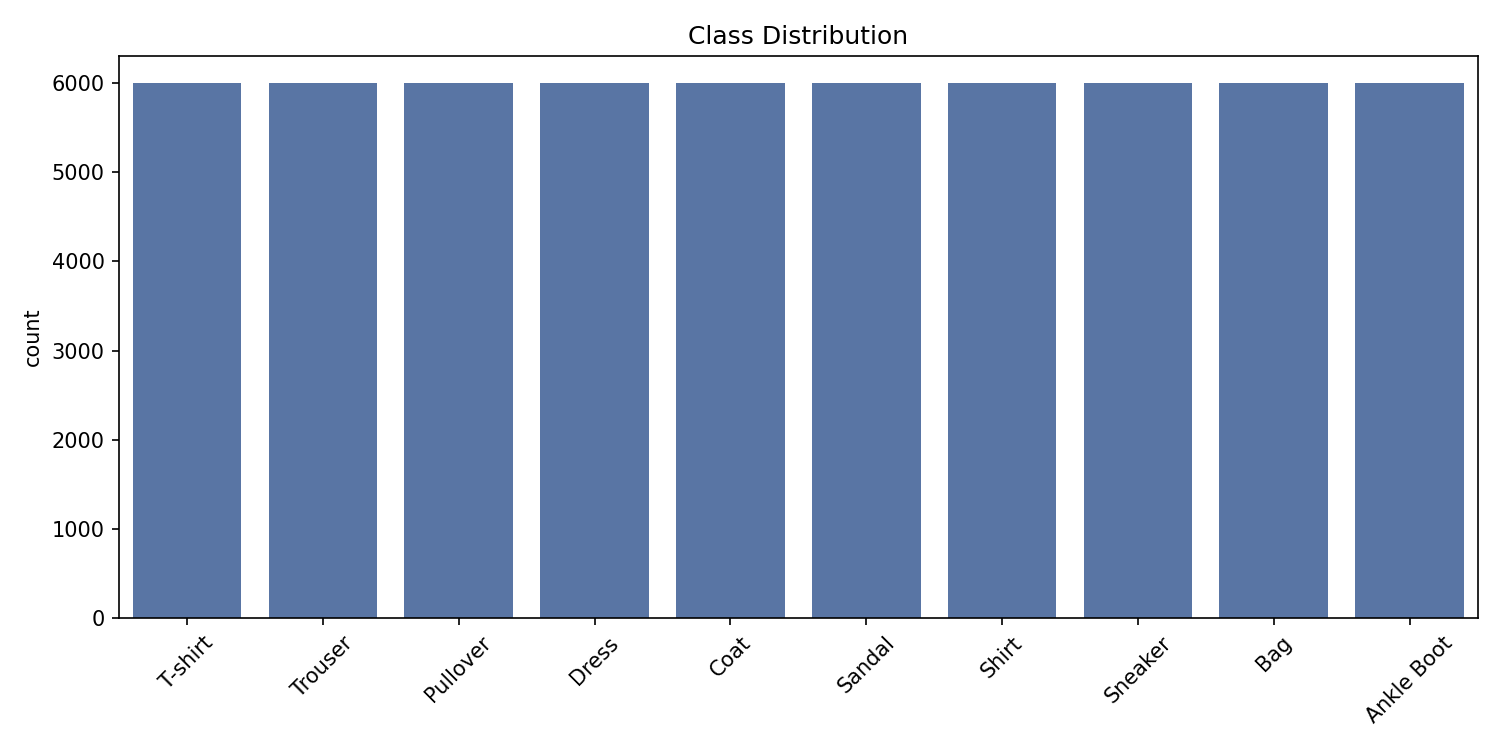
\includegraphics[width=0.7\textwidth]{figs/fig2_class_distribution.png}
\caption{Class distribution of the training set.}
\end{figure}

\textit{Inference:} All ten classes contain exactly 6,000 training images, so Fashion-MNIST is perfectly balanced. This means we don't need to worry about class-imbalance techniques (class weighting, oversampling, etc.) here, and it also means the weaker per-class scores for Shirt/Pullover/Coat genuinely reflect visual difficulty rather than one class simply having fewer training examples.

\subsection{Training Accuracy vs Epoch / Validation Accuracy vs Epoch}
\begin{figure}[h]
\centering
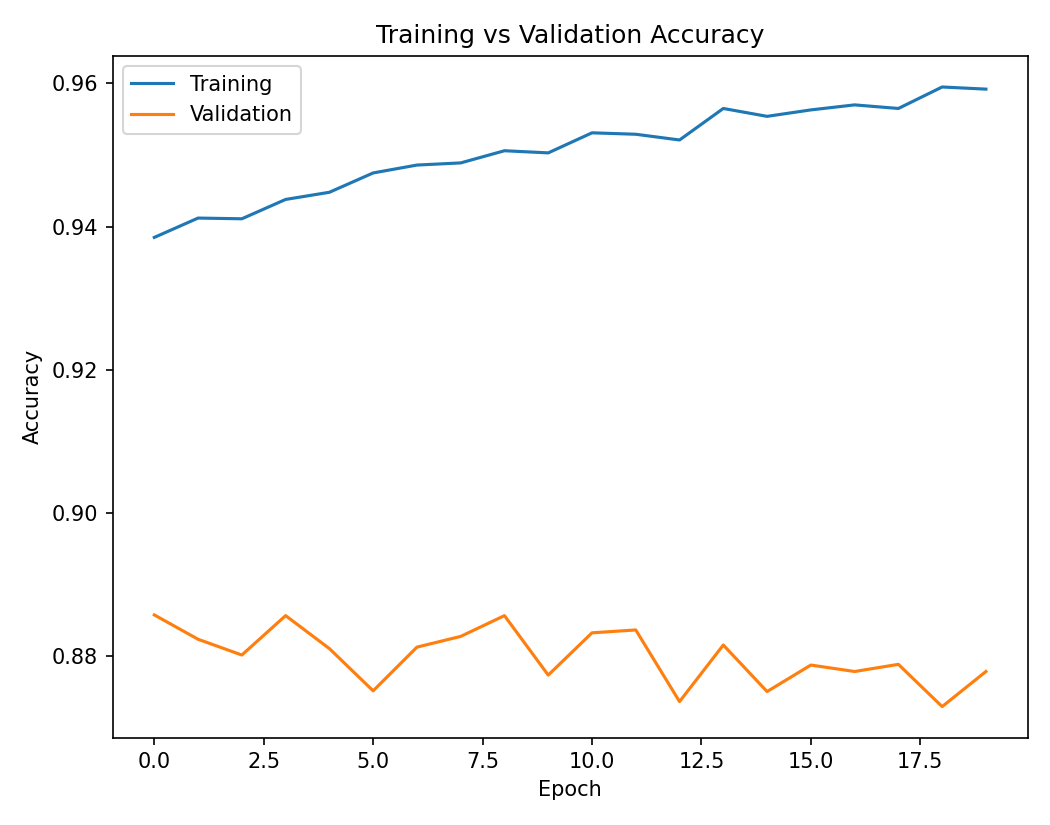
\includegraphics[width=0.65\textwidth]{figs/fig3_accuracy.png}
\caption{Training and validation accuracy across 20 epochs.}
\end{figure}

\textit{Inference:} Training accuracy climbs smoothly and continuously toward 96\%, while validation accuracy jumps up quickly in the first epoch and then essentially flatlines (with some noisy up-and-down movement) around 87--88\% for the rest of training. The widening gap between the two curves after roughly epoch 8--10 is the clearest visual sign that the model is starting to overfit the training data rather than continuing to learn genuinely useful features.

\subsection{Training Loss vs Epoch / Validation Loss vs Epoch}
\begin{figure}[h]
\centering
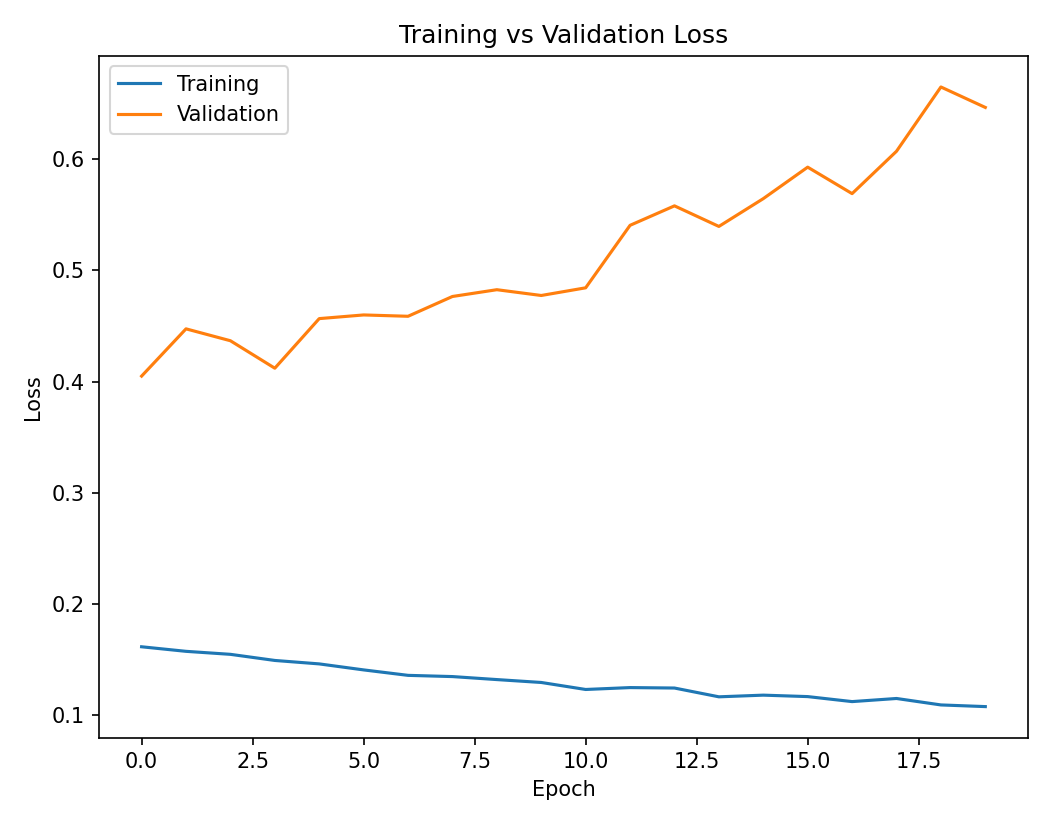
\includegraphics[width=0.65\textwidth]{figs/fig4_loss.png}
\caption{Training and validation loss across 20 epochs.}
\end{figure}

\textit{Inference:} Training loss decreases steadily throughout all 20 epochs, but validation loss bottoms out around epoch 3--4 and then rises fairly consistently afterward, nearly doubling by epoch 20. This divergence -- falling training loss alongside rising validation loss -- is the single strongest piece of evidence in this report that the baseline model is overfitting, and it suggests that early stopping around epoch 4--8, or adding regularization (dropout, weight decay), would likely give a model that generalizes better than training the full 20 epochs did.

\subsection{Confusion Matrix}
\begin{figure}[h]
\centering
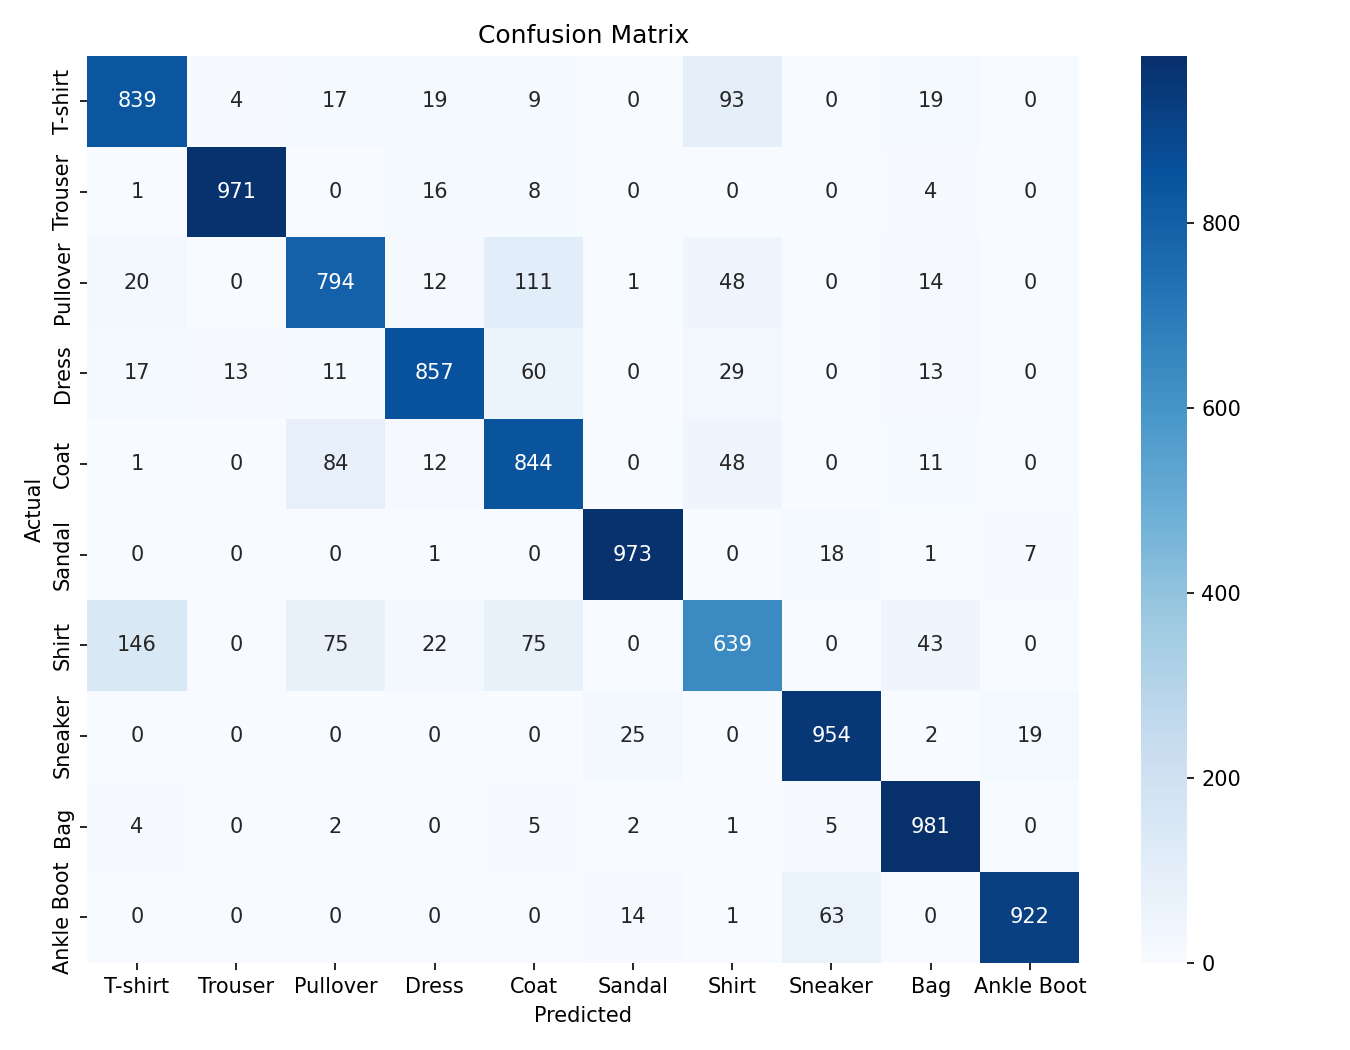
\includegraphics[width=0.75\textwidth]{figs/fig5_confusion_matrix.png}
\caption{Confusion matrix of the baseline model on the 10,000-sample test set.}
\end{figure}

\textit{Inference:} The matrix is strongly diagonal overall, confirming the 87.74\% accuracy, but there is a clearly visible block of confusion among Shirt, T-shirt, Pullover and Coat -- Shirt in particular gets misclassified as T-shirt and Coat noticeably often. In contrast, classes like Trouser, Bag, Sandal and Ankle Boot are almost perfectly separated from everything else, consistent with their high individual F1-scores in the classification report.

\subsection{Hyperparameter Search Results}
\begin{tcolorbox}[colback=gray!5, colframe=gray!60, title=\textbf{PLACEHOLDER -- Hyperparameter Search Results plot}]
The RandomizedSearchCV run did not finish executing (see Section 8.4), so \texttt{results["mean\_test\_score"]} was never populated and this plot (CV accuracy vs.\ search iteration) could not be generated. Paste the plot here once the search has been re-run to completion.
\end{tcolorbox}

\subsection{Best Model Accuracy Comparison}
\begin{tcolorbox}[colback=gray!5, colframe=gray!60, title=\textbf{PLACEHOLDER -- Baseline vs Optimized bar chart}]
This bar chart compares baseline accuracy against optimized accuracy, both of which depend on \texttt{random\_search.best\_estimator\_}. Since the search did not complete, optimized accuracy does not exist yet. Paste the plot here once the optimized model has been trained and evaluated.
\end{tcolorbox}

% =========================================================
\section{Results}

\subsection*{Best Hyperparameters}
\begin{center}
\begin{tabular}{|l|l|}
\hline
Hidden Layers & [TO BE FILLED AFTER RE-RUNNING SEARCH] \\
\hline
Hidden Neurons & [TO BE FILLED AFTER RE-RUNNING SEARCH] \\
\hline
Learning Rate & [TO BE FILLED AFTER RE-RUNNING SEARCH] \\
\hline
Batch Size & [TO BE FILLED AFTER RE-RUNNING SEARCH] \\
\hline
Optimizer & [TO BE FILLED AFTER RE-RUNNING SEARCH] \\
\hline
Activation Function & [TO BE FILLED AFTER RE-RUNNING SEARCH] \\
\hline
Epochs & [TO BE FILLED AFTER RE-RUNNING SEARCH] \\
\hline
Dropout & [TO BE FILLED AFTER RE-RUNNING SEARCH] \\
\hline
Cross-validation Accuracy & [TO BE FILLED AFTER RE-RUNNING SEARCH] \\
\hline
Testing Accuracy & [TO BE FILLED AFTER RE-RUNNING SEARCH] \\
\hline
\end{tabular}
\end{center}

\subsection*{Performance Comparison}
\begin{center}
\begin{tabular}{|l|l|l|}
\hline
\textbf{Metric} & \textbf{Baseline} & \textbf{Optimized} \\
\hline
Accuracy & 0.8774 & [PENDING] \\
\hline
Precision & 0.8772 & [PENDING] \\
\hline
Recall & 0.8774 & [PENDING] \\
\hline
F1-score & 0.8763 & [PENDING] \\
\hline
Training Time & $\approx$ 20 epochs, $\sim$8--10 s/epoch on the available runtime (see Section 8.2 log) & [PENDING] \\
\hline
\end{tabular}
\end{center}

The Baseline column above is filled in directly from Sections 8.2--8.3; the Optimized column is intentionally left as a placeholder pending a completed hyperparameter search run, as explained in Section 8.4.

% =========================================================
\section{Discussion}
\begin{enumerate}[label=\arabic*.]
    \item \textbf{Which optimization method was used?} RandomizedSearchCV (Scikit-learn) wrapping the Keras model via SciKeras' \texttt{KerasClassifier}, configured for \texttt{n\_iter=20} random hyperparameter draws with 5-fold cross-validation. Randomized Search was chosen over an exhaustive Grid Search specifically because the search space here is large (the grid defined in Section 7.7 has $3 \times 4 \times 3 \times 3 \times 3 \times 3 = 972$ possible combinations even before multiplying in batch size and epochs), and evaluating even a small random subset of that grid was already expensive enough that the run had to be interrupted -- a full grid search would have been far worse.

    \item \textbf{Which hyperparameters were selected?} Not yet known -- \texttt{random\_search.best\_params\_} was never populated because the search was interrupted before completion (Section 8.4). This should be filled in once the search has been re-run to completion.

    \item \textbf{Did optimization improve performance?} Cannot be answered yet for the same reason. Once the optimized model has been trained and evaluated, this should be compared directly against the baseline's 87.74\% test accuracy (Section 8.3) using the Performance Comparison table in Section 10.

    \item \textbf{Which hyperparameter had the greatest impact?} Also pending the completed search results (this is normally read off from \texttt{results["mean\_test\_score"]} sorted/grouped by each hyperparameter, or from the search-results plot in Section 9.6). Based on general MLP behaviour, however, we would expect learning rate and the choice of optimizer to matter the most for this architecture -- a learning rate of 0.1 combined with plain SGD, for instance, would likely train far worse than Adam at 0.001, purely because of how sensitive gradient descent is to step size on a loss surface like this one.

    \item \textbf{Compare Grid Search and Randomized Search.} Grid Search exhaustively evaluates every combination in the specified parameter grid, which guarantees finding the best combination within that grid but scales combinatorially -- with 8 hyperparameters and 3--4 candidate values each, a full grid here would run into the thousands of fits, which is computationally infeasible for a from-scratch Keras MLP trained on 60,000 images. Randomized Search instead samples a fixed number of random combinations (\texttt{n\_iter=20} here) from the same space, trading the guarantee of finding the absolute best combination for a search cost that is fixed and controllable in advance. In practice, randomized search is usually the more sensible default for large search spaces like this one, since research has repeatedly shown it finds solutions close to the grid-search optimum at a small fraction of the compute cost -- which is exactly why the lab handout recommends it here.

    \item \textbf{Recommend the best MLP configuration.} Pending the completed search. As an interim recommendation based on the baseline results alone: given how clearly the model overfits after roughly epoch 8 (Section 9.4), a smaller number of epochs (or early stopping) combined with a non-zero dropout rate would likely be a better starting point than the raw baseline configuration, even before the full hyperparameter search results are available.
\end{enumerate}

% =========================================================
\section{Report Contents}
This report includes: Objective, Background Theory, Dataset Description, Image Preprocessing, Experimental Procedure, Source Code, Hyperparameter Optimization, Experimental Results, Mandatory Plots with Inference, Results Tables, Discussion, Conclusion and References.

% =========================================================
\section{Conclusion}
In this experiment we built and trained a Multi-Layer Perceptron on the Fashion-MNIST dataset, moving beyond the single-layer, linearly-separable-only perceptron of Experiment 1 to a network with two hidden layers, ReLU activations and a Softmax output. After flattening and normalizing the $28 \times 28$ images and one-hot encoding the ten class labels, the baseline architecture ($784 \rightarrow 128 \rightarrow 64 \rightarrow 10$, 109,386 trainable parameters) reached 87.74\% test accuracy, 87.72\% weighted precision, 87.74\% weighted recall and an F1-score of 87.63\% after 20 training epochs. The accuracy and loss curves made it clear that the model overfits fairly noticeably after around epoch 8, since training loss keeps falling while validation loss climbs -- a useful reminder that "train for more epochs" is not automatically better once the model has stopped learning genuinely new, generalizable structure. The confusion matrix and per-class report both pointed to the same weak spot: visually similar upper-body garments (Shirt, T-shirt, Pullover, Coat) are the classes the model struggles with most, which lines up with what a human would expect just from looking at the sample images.

The automated hyperparameter optimization stage (RandomizedSearchCV over hidden layers, neurons, learning rate, batch size, epochs, optimizer, activation and dropout) was set up correctly but the search run itself was interrupted before completion, so the "optimized" side of every comparison in this report -- best hyperparameters, optimized accuracy/precision/recall/F1, the search-results plot and the baseline-vs-optimized bar chart -- is left as an explicit placeholder rather than filled in with invented numbers. The code for the full search-and-retrain pipeline is included in Section 7 exactly as written and only needs to be re-run (ideally with a smaller search budget or more compute time) to populate the remaining tables and plots. Based on the overfitting pattern observed in the baseline model alone, a reasonable expectation is that the search will favour a configuration with some dropout and fewer effective training epochs (or early stopping) over the raw baseline setup, though this should of course be confirmed once actual search results are available.

% =========================================================
\section{References}
\begin{enumerate}
    \item I. Goodfellow, Y. Bengio and A. Courville, \textit{Deep Learning}, MIT Press, 2016.
    \item C. M. Bishop, \textit{Pattern Recognition and Machine Learning}, Springer, 2006.
    \item S. Haykin, \textit{Neural Networks and Learning Machines}, Pearson, 2009.
    \item Fashion-MNIST Dataset, Zalando Research, \url{https://github.com/zalandoresearch/fashion-mnist}.
    \item TensorFlow/Keras Documentation, \url{https://www.tensorflow.org/api_docs}.
\end{enumerate}

\end{document}
